\documentclass{jsarticle}
\usepackage{amssymb}
\usepackage{graphicx}
\usepackage[dvipdfmx]{color}
\usepackage{here}
\usepackage{tabularx}
\usepackage{amsmath}
\usepackage{url}
\usepackage[hang,small,bf]{caption}
\usepackage[subrefformat=parens]{subcaption}
\usepackage{tikz}
\usepackage{siunitx}
\usepackage{bm}
\usepackage{ascmac}
\usepackage{tikz}
\usepackage[top=15truemm,bottom=20truemm,left=20truemm,right=20truemm]{geometry}
\usetikzlibrary{shapes.geometric}
\usetikzlibrary {shapes.misc}
\usetikzlibrary{positioning}
\captionsetup{compatibility=false}

\usetikzlibrary{calc}
\usetikzlibrary{positioning}
\usetikzlibrary{arrows.meta}

\begin{document}


\rightline{2022/5/17}

\section*{Ex1.1}
(ブロックダイアグラム分解)
各入力$u$を下のように解$y$に写像するシステム$P_1$を考える。

\begin{equation}
  \left[\begin{array}{l}
  \dot{x}_{1} \\
  \dot{x}_{2}
  \end{array}\right]=\left[\begin{array}{cc}
  1 & 0 \\
  -1 & 2
  \end{array}\right]\left[\begin{array}{l}
  x_{1} \\
  x_{2}
  \end{array}\right]+\left[\begin{array}{l}
  4 \\
  1
  \end{array}\right] u, \quad y=\left[\begin{array}{ll}
  1 & 3
  \end{array}\right]\left[\begin{array}{l}
  x_{1} \\
  x_{2}
  \end{array}\right]
\end{equation}

このシステムを、以下のものだけで構成されるブロックダイヤグラムで表す。\\
・ 入力$u(\cdot)\in \mathbb{R}$を$\dot{y}=u$の解$y(\cdot)\in \mathbb{R}$に写像する、記号$\int$で表される積分系
\\
・ 入力ベクトル$u(\cdot)\in \mathbb{R}^k$をスカラー出力$y(t)=\sum^k_{i=1}u_i(t),\forall t \geq 0$に写像する、記号$\sum$で表される和算器\\
・ 入力$u(\cdot)\in \mathbb{R}$を出力$y(t) = \mathrm{g} u(t) \in \mathbb{R},$任意の$\mathrm{g}\in \mathbb{R}$について$ \forall t \geq 0$に写像する、
記号$\mathrm{g}$で表されるゲイン無記憶系\\


\begin{equation}
  \begin{aligned}
    y\; &=& x_1 &+& 3x_2 \\
    \dot{x_1} &=& x_1&+&&&  4u \\
    \dot{x_2} &=& -x_1 &+& 2x_2 &+& u\\
  \end{aligned}
\end{equation}




\begin{figure}[H]
  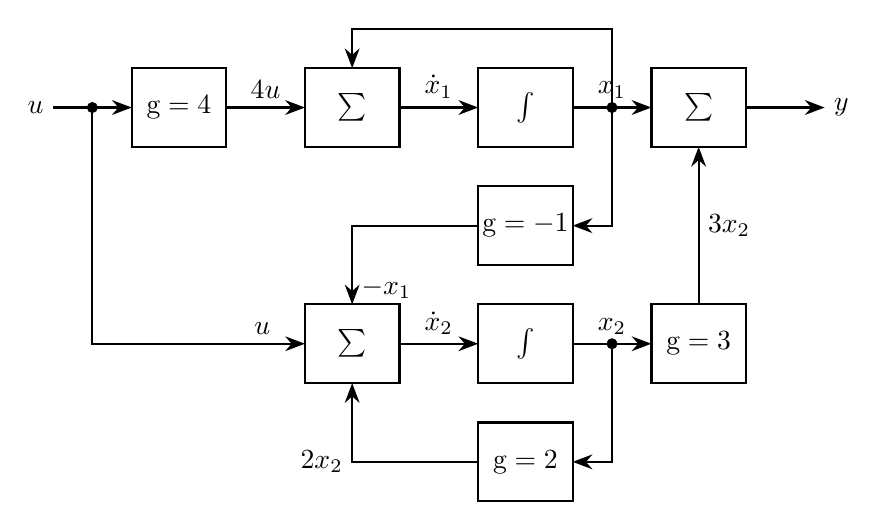
\begin{tikzpicture}
    [
    % 線と文字の間の間隔を設定
    every node/.style={outer sep=0.12cm, inner sep=0},
    % 矢印の設定
    arrow/.style={-{Stealth[length=0.25cm]}, thick},
    % ブロック
    block/.style={rectangle, draw, minimum height = 1cm,
    minimum width=1.2cm, thick, outer sep = 0},
    % 加え合わせ点
    sum/.style={thick, circle, draw, inner sep=0,
    minimum size=6pt, outer sep=0},
    % 引き出し点
    point/.style={radius=2pt}
    ]
    \node (r){$u$};
    \node [block, right=1 of r] (g4){$\mathrm{g=4}$};
    \node [block, right=1 of g4] (sum1){$\sum$};
    \node [block, right=1 of sum1] (int1){$\int$};
    \node [block, right=1 of int1] (sum3){$\sum$};
    \node [right=1 of sum3](y){$y$};
    \node [block, below=0.5 of int1] (g-1){$\mathrm{g=-1}$};
    \node [block, below=0.5 of g-1] (int2){$\int$};
    \node [block, right=1 of int2] (g3){$\mathrm{g=3}$};
    \node [block, left=1 of int2] (sum2){$\sum$};
    \node [block, below=0.5 of int2] (g2){$\mathrm{g=2}$};
    \fill [point]($(r.east)!0.5!(g4.west)$) circle coordinate (c1);
    \fill [point]($(int1.east)!0.5!(sum3.west)$) circle coordinate (c2);
    \fill [point]($(int2.east)!0.5!(g3.west)$) circle coordinate (c3);


    \draw[arrow] (r) -- (g4);
    \draw[arrow] (c1) |- (sum2)node [above, pos=0.9]{$u$};
    \draw[arrow] (g4) -- (sum1)node [above, pos=0.5]{$4u$};
    \draw[arrow] (sum1) -- (int1)node [above, pos=0.5]{$\dot{x}_1$};
    \draw[arrow] (int1) -- (sum3)node [above, pos=0.5]{$x_1$};
    \draw[arrow] (sum3) -- (y);
    \draw[arrow] (c2) |- (g-1);
    \draw [arrow] (c2) -- +(0, 1) -| (sum1);
    \draw[arrow] (g-1) -| (sum2)node [right, pos=0.9]{$-x_1$};
    \draw[arrow] (sum2) -- (int2)node [above, pos=0.5]{$\dot{x}_2$};
    \draw[arrow] (int2) -- (g3)node [above, pos=0.5]{$x_2$};
    \draw[arrow] (c3) |- (g2);
    \draw[arrow] (g2) -| (sum2)node [left, pos=0.5]{$2x_2$};
    \draw[arrow] (g3) -- (sum3)node [right, pos=0.5]{$3x_2$};

    % \draw[arrow] (sum) -- (K);
    % \draw[arrow] (K) -- (G) node [above, pos=0.5] {$u$};
    % \draw[arrow] (G.east) -- +(2, 0) node[right]{$y$};
    % \draw[arrow] (sum.west)+(-1, 0) node[left]{$r$} -- (sum.west)
    % node[below, xshift=-10pt]{$+$};
    % \fill [point] (G.east)+(1, 0) circle coordinate (y);
    % \draw [arrow] (y) -- +(0, -1) -| (sum) node[left, yshift=-15pt] {$-$};
  \end{tikzpicture}
\end{figure}


\end{document}